\documentclass[a4paper,12pt]{article}
\usepackage{algorithm}
\usepackage{algorithmic}
\usepackage{amsmath, amsthm, amsfonts}
\usepackage{graphicx}

\makeatletter
\renewcommand\paragraph{\@startsection{paragraph}{4}{\z@}%
  {-3.25ex\@plus -1ex \@minus -.2ex}%
  {1.5ex \@plus .2ex}%
  {\normalfont\normalsize\bfseries}}
\makeatother

\title{Creating a finite automaton to detect reduced words in coxeter groups}
\author{David Tyler}
\date{\today}

\begin{document}
\maketitle
\newpage

\setcounter{tocdepth}{1}
\tableofcontents
\newpage

%Set up the different types of theorems and definitions that will be used throughout the document.
\newtheorem{thm}{Theorem}[section]
\newtheorem{prop}[thm]{Proposition}
\newtheorem{cor}[thm]{Corollary}
\newtheorem{lem}[thm]{Lemma}
\newtheorem{example}[thm]{Example}

\theoremstyle{definition}
\newtheorem{definition}[thm]{Definition}

\section{Introduction}
This project is concerned with the word reduction problem in group theory. A non-technical way to look at it would be to say that if we are given a string of letters and some rules about which combinations of those letters can be ignored, can we quickly determine whether the string that we were given is as short as possible. If it isn't is there a quick way to make it shorter? Specifically for the sake of this project we are concerning ourselves with that problem for a small class of groups which are common throughout various branches of mathematics.

The aim of the project is to provide a thorough introduction to the techniques used in solving the word reduction problem for finitely generated coxeter groups. More specifically, as part of the project a program has been written which generates a finite state automaton that can detect reduced words in these groups. This document will begin by giving a brief background introduction to the notion of a coxeter group and its root system. Various examples of the different sorts of groups that can arise are given. Moving on from there the notion of dominance and minimal roots will be introduced and examples will be given of groups in which the minimal root system is not equal to the root system. This will lead into the significant results which allow the construction of the automaton and the algorithm to reduce words.

The last section of the project will discuss the algorithm and data structures in more technical detail with an aim of giving some idea of the computational complexity of the problem.

The first sections of this project follow more or less exactly the lecture notes of Howlett \cite{howlettnotes}. Arguments have been reordered, reworked and fleshed out to make them more understandable but in general the work is not original. The reason for this is that his aim in the lecture course seems to have been to prove the construction of the automaton that we programmed for this project and his work is by far the most direct way to arrive at these things. The last two sections deal more with the actual implementation and are nearly entirely my own work. Where this is not true references are given as is standard practice.

\subsection{What will not be covered?}
The assumption is that anyone reading this document will have a solid background in basic group theory and so certain notions which are not needed in any great depth will simply be stated. For example, the definition of a coxeter group uses the notion of a group presentation, however no definition of presentations will be given in this document. For basic information any undergraduate course on group theory will suffice.

The algorithm which the mathematics in this document leads up to involves the use of finite state automata, however no significant results about automata are used in this document so for a rigorous treatment of these objects the reader is referred to a text such as \cite{automata}.

Typically when one considers coxeter groups from a graduate level perspective it is useful to first study finite reflection groups and particularly to attack coxeter groups from a geometrical view. This is what is done in the canonical text by Humphreys \cite{humphreys90} and in most other books and articles. However, as the aim of this project is far more specific, we are not going to study the geometrical notions behind coxeter groups but rather consider them as objects acting on an abstract vector space. This is a far more productive way to arrive at results about infinite coxeter groups as geometrical intuition is often not sufficient for these groups.

\subsection{A look at the word reduction problem for a more simple example}
As alluded to earlier the problem of determining whether a word in a given group is reduced is non-trivial. Fortunately for us in most cases we are only interested in specific classes of groups in which the problem is more understandable. The simplest such example is the class of free groups.

In essence the question can be formulated as follows:
Given a group $G$ and a string of symbols $\left\{x_i\right\}_{i=1}^n \in G$ is there another such string of symbols $\left\{y_j\right\}_{j=1}^m \in G$ such that $m < n$ and $x_1 \ldots x_n = y_1 \ldots y_m$. 

Given a word $w = a_1^{\epsilon_1} a_2^{\epsilon_2} \ldots a_n^{\epsilon_n}$ where $\epsilon_i \in \left\{-1, 1 \right\}$ we can remove any pair of elements $a_i a_i^{-1}$ (by definition of the free group).

So a brute force algorithm to detect reduced words in the free group of order n ($F_n$) would be as follows:
\begin{algorithmic}[1]
	\STATE $reduced = true$
  \FOR{$index = 1$ to $n$}
		\IF{$w[index - 1] == w[index]^{-1}$}
			\STATE $reduced = false$
		\ENDIF
	\ENDFOR
	\RETURN $reduced$
\end{algorithmic}

Clearly this completes in linear time on the number of elements in the generating set of $F_n$. It is also fairly obvious that a similar algorithm which removes pairs of 'inverse' elements and then restarts would be in $P$ and more specifically would have a bound of $n^2$.

However, that is a fairly trivial example. In all cases, a word in the free group can easily be reduced by a human being without a significant amount of work.

\section{Definitions and Examples}

We begin by defining the notion of a coxeter group and giving 2 examples to illustrate what they are.

\begin{definition}
A group $G$ is a Coxeter group if it has a presentation in the form:
\begin{equation}
	G = \left\langle \left\{a \in \Sigma \right\} \: | \: a^2 = (ab)^{n_{ab}} = 1 \; \forall \; a, b \in \Sigma \; a \neq b\right\rangle
\end{equation}

In this definition $n_{ab} = n_{ba} \in \left\{2,3,4,\ldots\right\} \cup \infty$. $\left(ab\right)^{\infty} = 1$ is interpreted as meaningless in terms of group relations as it does not add any extra restrictions on words in the group.
\end{definition}

Essentially those groups of this form which have finite order can be thought of as groups of reflections. In fact, although that is not the aim of this essay, finite coxeter groups (i.e. those with finite order) are in bijection with the finite euclidean reflection groups. For a proper discussion on these topics see \cite{humphreys90}. The aims of this essay are geared more towards infinite coxeter groups where simple techniques will no longer work but examples are often taken from finite groups to aid simplicity.

We illustrate the notions with a trivial example:

\begin{example}
Let $A_2$ be the group with presentation: $\left\langle a, b | a^2, b^2, (ab)^3\right\rangle$

The elements of $A_2$ are $\left\{1, a, b, ab, ba, aba\right\}$ and they have a multiplication table:
\[ \left( \begin{array}{ccccccc}
	    & \textbf{1}   & \textbf{a}   & \textbf{b}   & \textbf{ab}  & \textbf{ba}  & \textbf{aba} \\
	\textbf{1}   & 1   & a   & b   & ab  & ba  & aba \\
	\textbf{a}   & a   & 1   & ab  & b   & aba & ba \\
	\textbf{b}   & b   & ba  & 1   & aba & a   & ab \\
	\textbf{ab}  & ab  & aba & a   & ba  & 1   & b \\
	\textbf{ba}  & ba  & b   & aba & 1   & ab  & a \\
	\textbf{aba} & aba & ab  & ba  & a   & b   & 1
\end{array} \right)\]

Now, we can also write the coefficients of the group presentation into a $n*n$ matrix where $n = \left|\Sigma\right|$. This is known as the coxeter matrix and uniquely determines the coxeter group. It can therefore be useful when a presentation is overly complicated (e.g. when inputting groups into a computer).

To illustrate this the coxeter matrix for $A_2$ is:

\[ \left( \begin{array}{cc}
1 & 3 \\
3 & 1
\end{array} \right) \]

Note in particular that the matrix is symmetric since if a word $w = a_1a_2 \ldots a_n = 1$ then by multiplying both side by $a_n$ and then $a_{n-1}$ etc we see that $v = a_na_{n-1} \ldots a_1 = 1$ also.

We can use the coxeter matrix defined in this manner as the incidence matrix for a graph. To do this let each generator correspond to a single generator and connect vertices in the following manner:

\begin{itemize}
	\item If $n_{ab} = 2$ then do not connect $a$ and $b$.
	\item If $n_{ab} = 3$ then connect $a$ and $ab$ but do not label the edge.
	\item If $n_{ab} > 3$ then connect $a$ and $b$ and label the edge with the value $n_{ab}$.
\end{itemize}

So the graph for the group $A_2$ is below:

\begin{figure}[H]
	\centering
		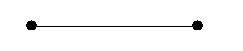
\includegraphics[width=50mm]{A_2.png}
	\label{fig:A_2}
\end{figure}

We will make extensive use of these different descriptions of the group throughout the document. Essentially however, they all just encode the same information about the group and are useful mainly as ways to visualise specific aspects of a group.
\end{example}

It is possible to construct much more complex examples as we have given ourselves no constraints on the number of generators yet. An example with 4 generators is as follows:

\begin{example}
Let 
\begin{align*}
	W = \langle& a,b,c,d \: | \: a^2 = b^2 = c^2 = d^2 \\
	&= (ab)^4 = (ac)^2 = (ad)^8 = (bc)^3 = (bd)^6 = (cd)^2 = 1\rangle
\end{align*}
	
This is a coxeter group from our definition above however it will be very difficult to determine anything useful about it simply from that presentation. It has the following coxeter matrix:
	
\[ \left( \begin{array}{cccc}
1 & 4 & 2 & 8 \\
4 & 1 & 3 & 6 \\
2 & 3 & 1 & 2 \\
8 & 6 & 2 & 1
\end{array} \right) \]

Using this matrix in the manner described above gives us the following graph:

\begin{figure}[H]
	\centering
		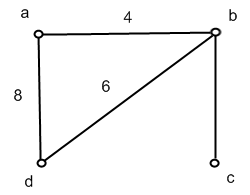
\includegraphics[width=50mm]{rand_graph.png}
	\label{fig:rand_graph}
\end{figure}

\end{example}

\section{Creating a Root System on Coxeter Groups}
We now develop what is known as the root system for a coxeter group (note that nothing in this section restricts the group to be finite). The notion of root system here is slightly different from the notion used in the study of Lie algebras although this should be clear as we proceed.

First, let V be a vector space over $\mathbb{R}$ with basis $\Pi = \left\{v_a \: | \: a \in \Sigma\right\}$, thus the basis is in bijection with the generating set of $W$.
Now we can define a bilinear symmetric product on this vector space by defining it on the basis elements as below:

\begin{equation*}
	\left(v_a \: . \: v_b\right) = 
	\begin{cases}
		1 & \text{if $a = b$}, \\
		-\cos{\frac{\pi}{n_{ab}}} & \text{if $a \neq b$}
	\end{cases}
\end{equation*}

This is positive definite provided that $n_{ab} \neq \infty$. In the case that $n_{ab} = \infty$ we say that $\left(v_a \: . \: v_b\right) = -1$.

Now with that bilinear product and given $v_a \in \Pi$ we can define a function $\rho_a : V \rightarrow V$ by:

\begin{equation*}
	\rho_a(v) = v - 2(v \: . \: v_a)v_a
\end{equation*}

The following proposition describes the properties of these functions.

\begin{prop}
	Given elements $v_a, v_b \in \Pi$ the function $\rho_a$ satisfies the following properties:
	\begin{enumerate}
		\item $\rho_a\left(v_a\right) = -v_a$
		\item $\rho_a ^ 2 = 1$
		\item $\left(\rho_a\rho_b\right) ^ {n_{ab}} = 1$
		\item The functions $\rho_a$ preserve the bilinear product.
	\end{enumerate}
\end{prop}

\begin{proof}
	With notation as in the proposition let $v$ be an arbitrary element of $V$. Then we prove part $1$ as follows:
	\begin{align*}
		\rho_a(v_a) &= v_a - 2\left(v_a \: . \: v_a\right)v_a \\
		&= v_a - 2v_a = -v_a
	\end{align*}
	
	Using this we can prove part $2$:
	\begin{align*}
		\rho_a^2(v) &= \rho_a(\rho_a(v)) \\
		\rho_a(v) &= v - 2\left(v \: . \: v_a\right)v_a \\
		\rho_a(\rho_a(v)) &= \rho_a(v) - 2\left(v \: . v_a\right)\rho_a(v_a) \\
		&= v - 2\left(v \: . \: v_a\right)v_a + 2\left(v \: . \: v_a\right)v_a \\
		&= v \text{ as required.}
	\end{align*}
	
	Part $3$ of the proposition is not difficult to prove but the proof is longer and more involved than the above so is omitted. For the interested reader, a proof of this can be found in the lecture notes of Howlett \cite{howlettnotes}
	
	Part $4$ of the proposition is another simple calculation:
	
	\begin{align*}
		\left(\rho_a(v) \: . \: \rho_a(u)\right) &= ((v - 2(v \: . r_a)r_a) \: . \: (u - 2(u \: . \: r_a)r_a)) \\
		&= (v \: . \: u) - 2(v \: . \: r_a)(r_a \: . \: u) - 2(u \: . \: r_a)(v \: . \: r_a) + 4(v \: . \: r_a)(u \: . \: r_a)(r_a \: . \: r_a) \\
		&= (v \: . \: u)
	\end{align*}
	
	showing that the binary product is indeed preserved under these functions.
\end{proof}

Having shown that these functions satisfy all of the relations in the group $W$ we know from representation theory that there exists a homomorphism from the group into the general linear group over the vector space $V$. We call this homomorphism $\rho: W \rightarrow GL(V)$ (the geometric representation) and define it as follows:

\begin{equation*}
	\rho(a) = \rho_a \ \forall \ a \in \Sigma
\end{equation*}

Moreover, since creating this we are now able to say that $W$ acts on the vector space $V$ by defining the action of the generators on an arbitrary element of the vector space:

\begin{equation*}
	av = v - 2(v \: . \: v_a)v_a \: \forall a \in \Sigma, v \in V
\end{equation*}

This is associative (necessary in order for it to be an action) because 

\[(ab)v = \rho_{ab}(v) = \rho(ab)(v) = \rho(a)\rho(b)(v) = \rho_a(\rho_b(v))\].

Also the group identity sends vectors to themselves as required; 

\[1v = aav = \rho_a^2(v) = v\] by the proposition. 

As a result of the work we are about to do we will prove that this action is in fact faithful. Before we move, briefly taking stock of what has been achieved so far; we note that we have created a vector space whose basis is in bijection with the generating set of our group. We then set up an action of the group on this vector space which preserves some useful properties. 

Following on from this we now build the root system of the group. This is an object which is embedded in the vector space $V$ and turns out to be very useful for investigating a coxeter group $W$.

\begin{definition}
	The root system of $W$ is the set $\Phi \subset V$, 
	\[\Phi = \left\{ wv_a \: | \: w \in W, a \in \Sigma\right\}\]
\end{definition}

Note in particular that this set need not be finite as in the conventional definition of a root system. In fact as we will show, it is finite if and only if the group $W$ is finite. 

Since $\Phi$ lies in $V$ we can write elements of $\Phi$ as linear combinations of the basis vectors $v_a$.

The above definition of the root system tells us precisely how to calculate the root system of a given group. The key point to note is that the root system is closed under the action of the generators of $W$. This is clear from the definition of a root system and leads us to the following algorithm:

\begin{algorithmic}[1]
	\REQUIRE root list as list of roots, $v \in V$ as input.
	\FOR{each generator $a \in \Sigma$}
		\IF{$av \notin$ root list}
			\STATE root list = root list + $\left\{av\right\}$
			\STATE Call function again with new root list and $av$ as arguments.
		\ENDIF
	\ENDFOR
\end{algorithmic}

This essentially says that we can recursively build the root list by starting with the simple roots and performing actions of generators on them until no more roots can be found. Then since the root list is closed under the action of the generators we have the complete root list.

\subsection{Examples of calculating the root system}
To finish this section a few examples are given illustrating this approach to creating the root systems for specific groups.

\begin{example}
We begin with the very basic group that was used earlier ($A_2$). Its coxeter matrix was: 
	
\[ \left( \begin{array}{cc}
1 & 3 \\
3 & 1
\end{array} \right) \]

So we have that $(v_a.v_b) = -0.5$ and we already know the result of the scalar product of $(v_a.v_a)$ for any generator $a$. Therefore, starting with $a$ we begin building the root system in the manner described above.

\begin{algorithmic}[1]
	\STATE root list = $\left\{\right\}$
	\STATE $v = v_a$
	\STATE root list $= \left\{v_a\right\}$
	\STATE $v = av_a = -v_a$
	\STATE root list $= \left\{v_a, -v_a\right\}$
	\STATE $v = a(-v_a) = v_a$ \COMMENT {Already an element of the root list so we skip this one.}
	\STATE $v = b(-v_a) = -(v_a - 2(v_a.v_b)v_b) = -v_a - v_b$
	\STATE root list $= \left\{v_a, -v_a, -v_a - v_b\right\}$
	\STATE $v = a(-v_a - v_b) = v_a - av_b = v_a - (v_b - 2(v_a.v_b)v_a) = -v_b$
	\STATE root list $= \left\{v_a, -v_a, -v_a - v_b, -v_b\right\}$
	\STATE $v = a(-v_b) = -v_a - v_b$ \COMMENT {Already an element of the root list so skipped.}
	\STATE $v = b(-v_b) = v_b$
	\STATE root list $= \left\{v_a, -v_a, -v_a - v_b, -v_b, v_b\right\}$
	\STATE $v = av_b = v_a + v_b$
	\STATE root list $= \left\{v_a, -v_a, -v_a - v_b, -v_b, v_b, v_a + v_b\right\}$
	\STATE $v = a(v_a + v_b) = v_b$
	\STATE $v = b(v_a + v_b) = v_a$ \COMMENT {Since neither a nor b produced a new element we backtrack.}
	\STATE $v = b(-v_b) = v_b$ \COMMENT {Again nothing new is found so we backtrack.}
	\STATE $v = b(-v_a) = -v_a - v_b$ \COMMENT {Again nothing new is found so we backtrack.}
	\STATE $v = b(v_a) = v_a + v_b$ \COMMENT {Nothing new in the final backtrack so we start again with the other simple root.}
	\STATE $v = a(v_b) = v_a + v_b$
	\STATE $v = b(v_b) = -v_b$	
\end{algorithmic}

The algorithm then exits having completed the entire root list. There is clearly some redundancy here where roots are revisited many times and this is something that the software seeks to avoid where possible. The final root list is :

\[\left\{v_a, -v_a, -v_a - v_b, -v_b, v_b, v_a + v_b\right\}\]

Note in particular that it splits into positive and negative components where the negative components are simply the positive ones with negative sign.

\end{example}

\begin{example}
In this example we consider the group 

\begin{align*} 
	W = \langle a, b, c, d \: | \: a^2 = b^2 = c^2 = \\
	(ab)^3 = (ac)^2 = (ad)^3 = (bc)^3 = (bd)^2 = (cd)^3\rangle. 
\end{align*}

This groups has coxeter matrix:

\[ \left( \begin{array}{cccc}
1 & 3 & 2 & 3 \\
3 & 1 & 3 & 2 \\
2 & 3 & 1 & 3 \\
3 & 3 & 2 & 1
\end{array} \right) \]

and therefore, $(v_a.v_b) = (v_a.v_d) = (v_b.v_c) = (v_c.v_d) = -0.5$, $(v_a.v_c) = (v_b.v_d) = 0$.

Using this we can generate a matrix consisting of the action of each generator on each simple root. The simple roots will form the columns and the generators the rows:

\[ \left( \begin{array}{cccc}
-v_a & v_b + v_a & v_c & v_a + v_d \\
v_a + v_b & -v_b & v_b + v_c & v_b \\
v_a & v_c + v_b & -v_c & v_c + v_d \\
v_d + v_a & v_b & v_d + v_c & -v_d \\
\end{array} \right) \]

Now consider the root $v_a + v_b$ generated as the action of $a$ on $v_b$. If we take the action of $c$ on that root we get $v_a + v_b + v_c$. Then taking the action of $d$ on that gives us $v_a + v_b + v_c + 2v_d$. In a similar way we can generate roots, $2v_a + v_b + v_c + v_d$, $v_a + 2v_b + v_c + v_d$ and $v_a + v_b + 2v_c + v_d$.

From there it is easy to see that simply following the algorithm we can build up a root system which will never end simply by applying $a$ then $b$ then $c$ then $d$. Each time all 4 generators have been used the coefficients of the simple roots in the result have gone up by 1. So after n iterations (of taking the action of all 4 generators) the result is $nv_a + nv_b + nv_c + (n + 1)v_d$. Clearly these are all distinct and therefore the root system for this group is infinite.
\end{example}

%Example 3 Infinite group (affine perhaps?)

\section{Properties of the Root System}
As can be seen from the examples in the previous section the root system seems to split into those roots which have positive coefficients and those which have negative components. This turns out to be a general fact and is stated in the below theorem:

\begin{thm}
\label{root_system_splits}
	Given a coxeter group $W$ with generating set $\Sigma$, if $v \in \Phi$ is a root in the root system of $W$ then $v$ can be written as
	\[v = \sum_{a \in \Sigma}\lambda_av_a\]
	Where $v_a$ are the simple roots (the basis vectors of the root system) and $\lambda_a \in \mathbb{R}$. These $\lambda_a$ are either ALL positive or ALL negative.
\end{thm}

In order to prove this theorem we first introduce the notion of length in a coxeter group. 

Given a word $w$ in the group, $w$ can be written as $w = a_1a_2 \ldots a_l$ for some collection $a_1, a_2, \ldots, a_k \in \Sigma$. This is clearly not unique as adding $a_1a_1$ to the end of the word produces the same element of the group $W$. We define the notion of the length of $w$ as follows:

\begin{definition}
	Given a coxeter group $W$ with generating set $\Sigma$ and a word $w \in W$ we say that the length of $w$ is defined as
	\[l(w) = min\left\{k > 0 | w = a_1a_2 \ldots a_k\right\}\]
\end{definition}

This is really just formalising the intuitive notion of the length of a word. We are saying that the length of a word in the group is the smallest number of characters which represent the same element of the group. However, this notion is by no means unique. A simple example in the group $A_2$ is seen by taking the relation between $a$ and $b$ and splitting it. 
\begin{align*}
	(ab)^3 = 1 \\
	ababab = 1 \\
	aba = bab
\end{align*}
And both $aba$ and $bab$ are reduced words in the group with the same length. In fact, there is a similar automata to the one developed in this project which will always reduce words into their lexographically least form (i.e. $a$ comes before $b$). 

Now that we have a formal notion of length in a coxeter group we can also formally define the notion of a reduced word in the group.

\begin{definition}
	Writing a word $w \in W$ in the form $w = a_1a_2 \ldots a_k$, the form is reduced if $k = l(w)$. Otherwise we say that the form is not reduced.
\end{definition}

The following proposition presents some trivial properties of the length function.

\begin{prop}
\label{prop_length_properties}
Given a coxeter group $W$ with generating set $\Sigma$, words $w, w' \in W$ and $a \in \Sigma$:
	\begin{enumerate}
		\item $l(w) = l(w^{-1})$
		\item $l(ww') \leq l(w) + l(w')$
		\item $l(ww') \geq l(w) - l(w')$
		\item $\vert{l(w) - l(wa)}\vert \leq 1$
		\item If $w \neq 1$ then $\exists a \in \Sigma$ such that $l(wa) = l(w) - 1$
	\end{enumerate}
\end{prop}

\begin{proof}
	\begin{enumerate}
		\item Given a representation of $w$ in terms of the minimum number of generators $w = a_1a_2 \ldots a_{l(w)}$ we can write $w^{-1} = a_{l(w)}a_{l(w) - 1} \ldots a_1$ and so $l(w^{-1}) \leq  l(w)$. Following an identical argument but swapping $w$ and $w^{-1}$ tells us that $l(w) \leq l(w^{-1})$ and therefore they are of equal length.
		\item Let $w = a_{i_1}a_{i_2} \ldots a_{i_{l(w)}}$ and $w' = a_{j_1}a_{j_2} \ldots a_{j_{l(w')}}$. Then \[ww' = a_{i_1}a_{i_2} \ldots a_{i_{l(w)}}a_{j_1}a_{j_2} \ldots a_{j_{l(w')}}\] Therefore $l(ww') \leq l(w) + l(w')$.
		\item Consider $l((ww')w'^{-1})$, from 2 this is, $l((ww')w'^{-1}) \leq l(ww') + l(w'^{-1})$. However, by 1 we know that $l(w'^{-1}) = l(w')$ and so we have $l(w) = l((ww')w'^{-1}) \leq l(ww') + l(w')$. Rearranging gives us $l(ww') \geq l(w) - l(w')$ as required.
		\item The inequality can be rewritten as $l(w) - 1 \leq l(wa) \leq l(w) + 1$. So by applying parts 2 and 3 which we have already proved this inequality is now a triviality.
		\item We already know from part 3 of the proposition that $l(wa) \geq l(w) - 1$. Now, given a representation of $w$ as $w = a_{i_1}a_{i_2} \ldots a_{i_{l(w)}}$, we choose $a = a_{i_{l(w)}}$. Since every generator is its own inverse in a coxeter group this implies that $wa = a_{i_1}a_{i_2} \ldots a_{i_{l(w)} - 1}$. So we have shown that $l(wa) \leq l(w) - 1$ and therefore they are equal.
	\end{enumerate}
\end{proof}

As stated earlier that proposition is essentially trivial, however it serves to show us some of the constraints that adding generators has on a word. Essentially, it says that adding a generator does not drastically change the length. This is crucial and it is the discovery of which generators shorten a word and which lengthen it that we need the root table for and which will lead us on to the idea of how to generate the automaton for our group.

Now moving on to more difficult ideas we come back to proving the theorem stated at the beginning of this section. It will follow as a direct consequence from the following important result which ties together the root system and the length of words in the group.

\begin{thm}
\label{relate_length_roots}
	Given a coxeter group $W$ with root system $\Phi$, $w \in W$, $a \in \Sigma$ where $\Sigma$ is a generating set for $W$. Then $l(wa) \geq l(w) \Rightarrow wv_a \in \Phi$ has all positive coefficients when written as the sum of simple roots.
\end{thm}

We have nearly everything that we need in order to prove this theorem but we will break it up into some components and prove these individually.

The proof itself will go by contradiction. Let $G \subset W$ be the set of words in $W$ for which the theorem fails for some $a \in \Sigma$. Choose $w \in G$ such that $l(w) \leq l(w') \: \forall \: w' \in G$ and let $a$ be the generator in $\Sigma$ for which the theorem fails.

\begin{lem}
\label{finite_sequence_ws}
	There exists a finite sequence $w = w_0, w_1, \ldots, w_k$ for which $l(w_i) = l(w_{i-1}) - 1$.
\end{lem}

\begin{proof}
	We prove this by construction. To find such a sequence, first note that $w$ cannot be the identity element as if it was then the statement of the theorem would hold since $1v = v$ for all positive combinations of the simple roots in $\Phi$. In particular this would be true for the simple roots themselves as they are positive. Therefore we know that $l(w) \geq 1$ and we are in the situation described in part 5 of proposition \ref{prop_length_properties} which tells us that there exists some $b \in \Sigma$ such that $l(wb) = l(w) - 1$. Define, $w_1 = wb$.
	Then we can define our sequence as follows:
	
	\begin{equation*}
		w_{i+1} =
		\begin{cases}
			w_ia \text{   if i is odd.} \\
			w_ib \text{   if i is even.}
		\end{cases}
	\end{equation*}
	
	It is clear that if $i$ is even then $l(w_ia) \geq l(w)$ since the last character of $w_i$ is $a$ and likewise if $j$ is odd then $l(w_jb) \geq l(w)$ since the last character of $w_j$ is $b$.
	
	If at any point for some $i$ even $l(w_ib) \geq l(w)$ then stop the sequence at $i$ and let $k = i$. Likewise for $j$ odd, if $l(w_ia) \geq l(w)$ then let $k = j$.
	
	It remains to see that this will be a finite sequence. But this is obvious since at any point in the sequence, $l(w_i) = l(w) - i$ and since a word cannot have negative length the maximum value for $k$ is $l(w)$ which is finite.
\end{proof}

What can we determine about this sequence? Well the first thing is to note that as discussed, $k \leq l(w)$ and also that by the construction $l(w_ka), l(w_kb) \geq l(w_k)$. This is notable since $l(w_k) = l(w) - k$ and because $k \geq 1$ (as $w_1$ always exists in our sequence), by the minimality of $w$ in $G$ we have that $w_k$ satisfies the theorem. Thus $wv_a, wv_b$ are both roots with positive coefficients.

To aid notation for the next part we consider $w$ as the product of $w_k$ with an element of the group $x$ which is an alternating combination of $a's$ and $b's$. From our construction we know that $wbab\ldots = w_k$ and so $w = w_k\ldots ab$. Define $x = \ldots ab$. Then we know that $x$ ends in $b$ and alternates between $a$ and $b$. However, we do not know what the first element is or how long it is.

\begin{lem}
	A subgroup generated by 2 generators in a coxeter group is dihedral.
\end{lem}

\begin{proof}
	This is a triviality and holds simply by considering the presentation of a dihedral group as a coxeter group with 2 generators as is done in various sources (e.g. Kane's book in reflection groups \cite{kane01}).
\end{proof}

\begin{lem}
	$xv_a = \lambda v_a + \mu v_b$. Where $\lambda$ and $\mu$ are both positive.
\end{lem}

\begin{proof}
	In order to prove this we state without proof a result rooted more in geometrical arguments than algebraic. The matrix of $(ab)^m$ on the space spanned by the simple roots $v_a, v_b$ with respect to those simple roots is:
\[ \left( \begin{array}{cc}
\frac{\sin{(2m+1)\theta}}{\sin{\theta}} & -\frac{\sin{2m\theta}}{\sin{\theta}} \\ 
\frac{\sin{2m\theta}}{\sin{\theta}} & -\frac{\sin{(2m-1)\theta}}{\sin{\theta}}
\end{array} \right) \]

	Here we have defined $\theta = \frac{\pi}{n_{ab}}$, where $n_{ab}$ is the coefficient of the coxeter matrix for $a$ and $b$.

	Recall that $x \in W$ is made up of alternating $a$ and $b$ and so is either of the form $(ab)^{\frac{k}{2}}$ if $k$ is even or $(ba)^{\frac{k-1}{2}}b$ if $k$ is odd. So the action of $x$ on $v_a$ is given by:
	\begin{equation*}
		xv_a = 
		\begin{cases}
			(ab)^{\frac{k}{2}}v_a \text{ if k is even.} \\
			(ba)^{\frac{k-1}{2}}bv_a \text{ if k is odd.}
		\end{cases}
	\end{equation*}
	
	From the statement above we know that the value of $xv_a = \frac{\sin{(k+1)\theta}}{\sin{\theta}}v_a + \frac{\sin{k\theta}}{\sin{\theta}}v_b$ when $k$ is even. When $k$ is odd we note that 
	\begin{align*}
		(ba)^{\frac{k-1}{2}}bv_a &= (ba)^{\frac{k-1}{2}}b(-av_a) \\
		&= -(ba)^{\frac{k-1}{2}}bav_a \\
		&= -(ba)^{\frac{k}{2}}v_a \\
		&= \frac{\sin{(k+1)\theta}}{\sin{\theta}}v_a + \frac{\sin{k\theta}}{\sin{\theta}}v_b
	\end{align*}

	So it remains to see that the coefficients $\lambda = \frac{\sin{(k+1)\theta}}{\sin{\theta}}$ and $\mu = \frac{\sin{k\theta}}{\sin{\theta}}$ are both positive. $\sin{\theta} \geq 0$ for all the possible values of $n_{ab}$, and $\sin{(k+1)\theta} \geq 0$ if $k < n_{ab}$. $k$ was defined to be the length of $x$ and if $x$ has length greater than $n_{ab}$, since we are working in a dihedral group it is possible to find a smaller form of the same word as an alternating string of $a$ and $b$. 
	
	Furthermore, $(ab)^m = (ba)^m$ and so if $k = n_{ab}$ then $x$ would have a reduced expression ending with $a$. However, we showed prior to these lemmas that this could not be the case from the definition of $w_k$ and $x$. So we have proved that $k = l(x) < n_{ab}$.
	
	Putting this together with the previous calculations gives us the result that $\lambda, \mu \geq 0$ and the lemma is proved.
\end{proof}

Now that we have proved those lemmas the result comes easily to hand. Consider the action of $w$ on the simple root $a$ and recall that these were chosen to be a counter example to the theorem.

\[wa = w_kxa = w_k(\lambda a + \mu a) = \lambda w_k a + \mu w_k b\]

Then because of lemma \ref{finite_sequence_ws} we have $w_ka, w_kb$ as both positive roots and therefore $\lambda w_k a + \mu w_k b$ as a root with positive coefficients also. However, this is a contradiction as we chose $w, a$ so that $wa$ would not have all positive coefficients. In this manner the theorem is proved and we move on to its important corollaries.

\begin{cor}
	With the notation and assumptions from the theorem we also have that $l(wa) \leq l(w) \Rightarrow wv_a \in \Phi$ has all negative coefficients when written as the sum of simple roots.
\end{cor}

\begin{proof}
	Given $w$ and $a$ as above we have that $l(wa) \leq l(w)$. Therefore $l((wa)a) \geq l(wa)$, so now we can apply the above theorem to $wa$ and $a$. This tells us that since $l((wa)a \geq l(wa)$ we must have $(wa)v_a \in \Phi^+$. Now $(wa)v_a = w(av_a) = w(-v_a) = -wv_a \in \Phi^+$ and we can conclude that $wv_a \in \Phi^-$.
\end{proof}

This has the desired effect of proving theorem \ref{root_system_splits} stated at the beginning of this section. 

\begin{definition}
	We define 
	\[\Phi^+ = \left\{v = \sum_{a \in \Sigma} v_a\lambda_a \in \Phi \: | \: \lambda_a \geq 0 \right\}\] and 
	\[\Phi^- = \left\{v = \sum_{a \in \Sigma} v_a\lambda_a \in \Phi \: | \: \lambda_a \leq 0 \right\}\]
\end{definition}

Since every root (by definition) can be written as $wv_a$ for some word $w \in W$ and simple root $v_a \in \Phi$, we have shown that either $l(wa) \geq l(w)$ and therefore $wv_a \in \Phi^+$ or $l(wa) \leq l(w)$ and therefore $wv_a \in \Phi^-$. So every root is either in $\Phi^+$ or in $\Phi^-$. This is equivalent to the statement of the theorem.

Theorem \ref{root_system_splits} in and of itself does not seem to be particularly useful but we can draw two very prominent results from it immediately.

\begin{cor}
	The geometric representation is faithful.
\end{cor}

\begin{proof}
	We are trying to prove that $\rho: W \rightarrow GL(V)$ is faithful, or equivalently that $wv = v \: \forall \: v \in V \Leftrightarrow w = 1$.
	
	Assume such a $w$ exists and is not equal to the identity element in the group. Then $l(w) > 0$ so there exists an element $a \in \Sigma$ such that $l(wa) < l(w)$. Now by the previous corollary we can conclude that $wv_a \in \Phi^-$. However, by our assumption $wv_a = v_a$ and since $v_a$ is a simple root it is in $\Phi^+$. We have a contradiction and the kernel of $\rho$ must indeed be trivial.
\end{proof}

The fact that the representation is faithful gives us the useful fact that the root system is infinite if and only if the group itself is infinite. By the definition of the root system, we can see that if $W$ is finite then there are only finitely many values that $wv_a$ can take. The important thing here is that if $W$ is infinite then each $wv_a$ is distinct for a given $v_a$. This is true because if we had $w, w' \in W$ such that $wv_a = w'v_a$ then $w = w'$ as a direct result of the fact that the geometric representation is faithful.

The final result of this section tells us precisely the relationship between adding generators to a word and the length of the new word.

\begin{cor}
	\label{cor_relate_root_length}
	\begin{equation*}
		l(wa) = 
		\begin{cases}
			l(w) + 1 \text{ if } wv_a \in \Phi^+ \\
			l(w) - 1 \text{ if } wv_a \in \Phi^-
		\end{cases}
	\end{equation*}
\end{cor}

\begin{proof}
	Again the proof of this is very simple now that we have the result of the theorem. We have already shown in proposition 4.3 part 4 that $l(wa) \in \left\{-1, 0, 1\right\}$. And putting this in conjunction with theorem \ref{relate_length_roots} we conclude that:
	\begin{equation*}
		l(wa) = 
		\begin{cases}
			l(w) + (1 \text{ or } 0) \text{ if } wv_a \in \Phi^+ \\
			l(w) - (1 \text{ or } 0) \text{ if } wv_a \in \Phi^-
		\end{cases}
	\end{equation*}
	
	So it only remains to show that $l(wa) \neq l(w)$. However, if $l(wa) = l(w)$ then both $l(wa) \geq l(w)$ and $l(wa) \leq l(w)$ and so by theorem \ref{relate_length_roots} and its corollaries we know that $wv_a \in \Phi^+$ and $wv_a \in \Phi^-$, which is a contradiction and we are done.
\end{proof}

\section{Creating the Automaton}

In fact we actually have all of the information that we need to create an automaton however, as well will see shortly, it is not going to be finite. Before moving on we give a brief overview of the notion of automatons.

\begin{definition}
	Formally an automaton can be considered to be a quadruple:
	\[M = (A, Q, \tau, F)\]
	Where $A$ is an arbitrary alphabet, $Q$ is the set of states, $\tau$ is a transition function $\tau: Q \text{ x } A \rightarrow Q$ and $F$ is a set of end states.
\end{definition}

In our case this means that $A$ is the set of generators $\Sigma$ of whichever group we are interested in, $Q$ are the different states which the automaton can be in, $\tau$ is a function which takes a state from $Q$ and the next generator in the word (which will be an element of $A$) and sends us to another state. $F$ would typically be a subset of $Q$, however in our case it is simply going to be a distinguished state NO which will be reached whenever a word is not reduced.

In general an automaton is fed a stream of elements of $A$ one at a time, it begins at a predetermined state $q_0$ which is called the initial state and proceeds to move from state to state via the transition function $\tau$ until it either reaches a state from $F$ or runs out of data. We could create a trivial automaton as follows:

\begin{align*}
	A = \left\{0, 1\right\} \\
	Q = \left\{\left\{0\right\}, \left\{1\right\}\right\} \\
	\tau(q, a) = q \: AND \: a \\
	F = \emptyset
\end{align*}

This is a very simple automaton and can be illustrated by the following diagram.

\begin{figure}[H]
	\centering
		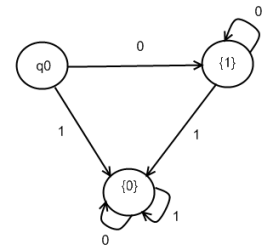
\includegraphics[width=73mm]{and_automaton.png}
	\label{fig:and_automaton}
\end{figure}

Note that some states return to themselves creating cycles in the automaton. There is also no formal requirement to have a finishing state although in the case we are interested in we will have one.

So what is it exactly that we are trying to accomplish? Well, the aim of this project is to produce a finite state automaton which recognises reduced words in a coxeter group. The original work done on this was in \cite{brinkhowlett93} where Brink \& Howlett proved that Coxeter groups are automatic and we follow the approach discussed there rather than later improvements.

Now if we are trying to recognise reduced words using an automaton, we are going to be given a word $w$ represented by a string of generators as input and asked to go through it generator by generator testing each to see if it reduces the size of the subword reached up to that point. This should remind us of a corollary proved at the end of the last section. We showed that adding a generator to the end of a word reduces the length of the word (by 1) if and only if the action of the word on the simple root of that generator is a negative root.

Therefore if we start with a word $w = a_1a_2 \ldots a_k$ and go from left to right we know that the subword $w_1 = a_1$ will definitely be reduced so we move on to the next generator. We ask whether the subword $w_2 = a_1a_2$ is reduced. It is not reduced if and only if $l(w_2) < 2$ which is true if and only if $a_1v_{a_2} \in \Phi^-$. However, $a_1v_{a_2} = v_{a_2} - 2(v_{a_2} \: . \: v_{a_1})v_{a_1}$. So since the action of $a_1$ on $v_{a_2}$ affects only the component of $v_{a_2}$ which is from the simple root $v_{a_1}$, then given that $(a \: . \: b) \leq 0$ for all simple roots $a, b$, we know that the new root will be positive if and only if the two generators are not equal.

In fact what we have done there is to show that for a generator $a \in \Sigma$. The only root which has the property $v \in \Phi^+$ and $av \in \Phi^-$ is $v = v_a$. We will use this many times throughout the rest of the document.

One could proceed in this manner going from generator to generator calculating the action of the subword $w_k = a_1 \ldots a_k$ on the simple root $v_{k + 1}$. If and only if the resulting root is positive do we have a reduced word. This certainly provides us with an algorithm to detect reduced words, however it is not a finite state machine and the number of calculations is a function of the length of the word (which might be very large). 

In order to find an automaton we introduce some new notation.

\begin{definition}
	Given a coxeter group $W$ with root system $\Phi = \Phi^+ \cup \Phi^-$ define for every word $w \in W$:
	\[N(w) = \left\{v \in \Phi^+ \: | \: wv \in \Phi^-\right\}\]
\end{definition}

\begin{lem}
	Given a word $w \in W$, and a generator $a \in \Sigma$ then if $l(wa) > l(w)$ we have that $N(wa) = aN(w) \cup \left\{v_a\right\}$.
\end{lem}

\begin{proof}
	First we show that $N(wa) \supseteq aN(w) \cup \left\{v_a\right\}$: Given $v \in aN(w) \cup \left\{v_a\right\}$, if $v = v_a$ then $av_a = -v_a$ and so $wav_a = w(-v_a) = -wv_a$ so either $v_a \in N(w)$ or $v_a \in N(wa)$. However, if $v_a \in N(w)$ then by corollary \ref{cor_relate_root_length} $l(wa) = l(w) - 1$ which would contradict the original assumption that $l(wa) > l(w)$. Therefore, $v_a \in N(wa)$. Now consider $v \in aN(w)$, so $v = ax$ for some $x \in N(w)$.
	
\[(wa)v = (wa)(ax) = wx\]

But $x \in N(w)$ so $wx \in \Phi^-$ and therefore $(wa)v \in \Phi^-$ giving us the result that $v \in N(wa)$ as required.

For the second part of the proof we will show that $N(wa) \subseteq aN(w) \cup {v_a}$: Given $v \in N(wa)$ we know that $(wa)v \in \Phi^-$. But $(wa)v = w(av) \in \Phi^-$ and so $av \in N(w)$. If $av \in \Phi^-$ then we have already shown that $v = v_a$ so either $av \in \Phi^+$ or $v = v_a$. Therefore, we get the result that either $v \in aN(w)$ or $v = v_a$ as required.
\end{proof}

\begin{prop}
	If $w = a_1a_2 \ldots a_k$ is a word such that $l(w) = k$ in a coxeter group $W$ with generating set $\Sigma$ then:
	\[N(w) = \left\{v_{a_k}, a_kv_{a_{k - 1}}, a_ka_{k - 1}v_{a_{k - 2}} \ldots, a_ka_{k - 1} \ldots a_2v_{a_1}\right\}\]
\end{prop}

\begin{proof}
	We will prove this by induction on the length of the word $w$.
	
	Case 1: If the length of the word is 1 then we know that the only root which sends $w = a_1$ to a negative root is the simple root $v_{a_1}$.
	
	Case $k$: We assume that the proposition holds for any word of length $k - 1$. Then given a word $w$ of length $k$ represented as $w = a_1a_2 \ldots a_{k-1}a_k$ it can be written as $w = w'a_k$ where $w' = a_1a_2 \ldots a_{k-1}$. Then $l(w') = k - 1$ and so we know $N(w')$ from the induction hypothesis. Now by the previous lemma $N(w'a_k) = a_kN(w') \cup \left\{v_{a_k}\right\}$. Rewriting this using the induction hypothesis we get:
	
	\begin{align*}
	N(w) = N(w'a_k) = a_k\{ & v_{a_{k-1}}, a_{k-1}v_{a_{k - 2}}, a_{k-1}a_{k - 2}v_{a_{k - 3}} \ldots, \\
	                        & a_{k-1}a_{k - 2} \ldots a_2v_{a_1}\} \cup \left\{v_{a_k}\right\}
	\end{align*}
	
	Multiplying into the set we get the formula required:
	
	\[N(w) = \left\{v_{a_k}, a_kv_{a_{k - 1}}, a_ka_{k - 1}v_{a_{k - 2}} \ldots, a_ka_{k - 1} \ldots a_2v_{a_1}\right\}\]
	
	and the conclusion is proved.
	
\end{proof}

Recall the notation previously used for the definition of the automaton:
\[M = (A, Q, \tau, F)\]

As explained earlier, the alphabet $A$ is going to be the set of generators $\Sigma$. The set of states $Q$ is going to be all combinations of roots from $\Phi^+$ plus one extra state which we will simply call 'No'. This extra state 'No' will also serve as the only element of $Q$ in $F$. The function $\tau: Q \text{ x } A \rightarrow Q$ is defined as follows:
\begin{equation*}
	\tau(S, a) = 
	\begin{cases}
		No \text{ if } a \in S \text{ or } S = No \\
		aS \cup \left\{v_a\right\} \text{ otherwise.}
	\end{cases}
\end{equation*}

The starting state is defined to be the empty set. Now note in particular that as in the example of the automaton described previously there is a state here which when entered is never left. That is the fail state ('No'). It is obvious that this should indeed be the case as if there is a subword of $w$ which is not reduced then the word itself cannot be reduced.

\begin{lem}
	The automaton given above recognises reduced words in a coxeter group $W$.
\end{lem}

\begin{proof}
	As this is the identical construction used by Brink \& Howlett we follow their proof of this more or less exactly. 
	
	The aim here is to prove that if we are given a word $w = a_1a_2 \ldots a_k$, which may or may not be reduced, then defining $w_i = a_1a_2 \ldots a_i$ we would like to show that the state which is arrived at after $a_i$ has been read is:
	\begin{equation*}
		S_i = 
		\begin{cases}
		No \text{ if } a_1a_2 \ldots a_i \text{ is not reduced.} \\
		N(w_i) \text{ if } a_1a_2 \ldots a_i \text{ is reduced.}
		\end{cases}
	\end{equation*}
	
	This is trivial for the case where $i = 0$ as the automaton is in the start state which is $S_0 = \emptyset$. We assume that the hypothesis holds for a word of length $i - 1$ and attempt to prove that it holds for a word of length $i$. As state previously, if a subword such as $w_{i-1}$ is not reduced then neither is $w_i$ so if $w_{i-1}$ is not reduced then we are done as $S_i = S_{i-1} = No$. We therefore assume that the subword $w_{i-1}$ is reduced, and therefore $S_{i-1} = N(w_{i-1})$. 
	
	Now consider two cases:
	
	Case 1: $v_{a_i} \in N(w_{i-1})$. Then by definition of $N$, $wv_{a_i} \in \Phi^-$ and so by corollary \ref{cor_relate_root_length} $l(wa) = l(w) - 1$ so $w_i$ is not reduced. Then by the definition of $\tau$ since $v_{a_i} \in S_{i-1} = N(w_{i-1})$, we have that $\tau(S_{i-1}, a_i) = No$.
	
	Case 2: $v_{a_i} \notin N(w_{i-1})$. We know that $a_1a_2 \ldots a_i$ is reduced and that $N(w_i) = a_iN(w_{i-1}) \cup \left\{v_{a_i}\right\}$. But this is equal to $a_iS_{i-1} \cup \left\{v_{a_1}\right\} = \tau(S_{i-1}, a_i) = S_i$ as required.
\end{proof}

So we have shown that there exists an automaton that detects reduced words in a Coxeter group. However, this automaton need not be finite. In fact it is only going to be finite when the root system is finite and we have already seen from one of the examples earlier that the root system need not be finite unless the group itself is. So although this automaton is fine for finite groups, there are already ways to quickly determine reduced words in a finite coxeter group so it is not useful. The breakthrough with this came as the result of the work by Brink \& Howlett in the earlier 90's where they showed that using the notion of dominant roots (we will also use the term minimal but the ideas are the same) that the automaton can be restricted to a finite number of states and the following theorem can be proved.

\begin{thm}
	For any coxeter group $W$ with generating set $\Sigma$ there exists a finite state automaton which detects reduced words in the group.
\end{thm}

\section{Minimal Root Systems}
In order to make the automaton finite we want to reduce the number of roots in the root system to be finite. To do that we introduce the notion of a minimal root and dominance on the root system.
	
\begin{definition}
	We say that given two roots $u, v \in \Phi^+$, $u \neq v$ $u$ dominates $v$ if $u \in N(w) \Rightarrow v \in N(w)$ for every $w \in W$. Now we define the following two sets:
	\[\Delta = \left\{ u \in \Phi^+ \: | \: u \text{ dominates some } v \in \Phi^+\backslash\left\{u\right\} \right\} \]
	\[\Delta' = \Phi^+\backslash\Delta\]
\end{definition}

We call $\Delta'$ the set of minimal roots.

\begin{thm}
	\label{minimal_root_set_finite}
	The set of minimal roots is finite for every coxeter group $W$.
\end{thm}

It is the view of those people who have studied this object over the last few years that this theorem is of a great deal of importance in and of itself rather than simply as a tool for generating the automaton. We will not prove the finiteness of the set of minimal roots in this project however for the interested reader the original proof can be found in the work of Brink \& Howlett \cite{brinkhowlett93}.

In order to show that there is no dominance in a finite group we introduce a relation on elements of the root system.

\begin{definition}
	Define the depth of a $v \in \Phi^+$ as \[dp(v) = min\left\{l \: | \: wv \in \Phi^-, l(w) = l\right\}\].
\end{definition}

\begin{lem}
\label{lem_dom_implies_depth}
	Given two roots $u, v \in \Phi^+$. $u$ dominates $v \Rightarrow dp(u) > dp(v)$.
\end{lem}

With this lemma we can show that the simple roots cannot dominate any element of the group; since for a simple root $v_a$, $av_a = -v_a$ and so $dp(v_a) = 1$. For all other roots, $dp(v) \geq 1$ thus simple roots cannot dominate anything.

\begin{proof}
	Begin by choosing $w \in W$ so that it fulfills the requirements for the definition of the depth of $u$. i.e. $wu \in \Phi^-$ and $l(w) = dp(u)$. Our aim is to find a specific element of $W$ such that its length is less than $w$ and it sends $v$ to a negative root.
	
	To do this we rewrite $w = aw'$ and note that $wu = (aw')u = a(w'u) \in \Phi^-$. Now since $l(w') < l(w)$ we cannot have $w'u \in \Phi^-$ so instead we have $w'u \in \Phi^+$ and therefore $w'u = v_a$ as that is the only root which $a$ sends negative. 
	
	However, we know that $u$ dominates $v$ and therefore $aw'v \in \Phi^-$ also. But then we have two cases. Either $w'v \in \Phi^+$ and then as above $w'v = v_a$. Or $w'v \in \Phi^-$ giving us $dp(v) \leq l(w') = l(w) - 1 < dp(u)$. We claim that $w'v \neq v_a$ as otherwise $w'v = w'u$ and therefore $u = v$ which cannot happen as $u$ dominates $v$.
\end{proof}

This lemma will form part of the proof of a proposition which allows us to generate the minimal root list easily.

With these definitions in mind we will restrict the automaton to be finite and then show that we have not lost any of the functionality. Essentially what we are going to do is ignore roots which are not minimal as they occur. The new definition of the automaton is:
\[M = (A, \hat{Q}, \hat{\tau}, No)\]

Where $\hat{Q}$ is defined as the set of all combinations of roots in $\Delta'$ and the new transition function is:

\begin{equation*}
	\hat{\tau(S, a)} = 
	\begin{cases}
		No \text{ if } a \in S \text{ or } S = No \\
		(aS \cup \left\{a\right\}) \cap \Delta' \text{ if } a \notin S
	\end{cases}
\end{equation*}

Now it is clear that if the set $\Delta'$ is finite (which we claim it is) then the set of all combinations of elements of $\Delta'$ is also going to be finite. Therefore the set of states is finite, and so we have created a finite state automaton. It remains to show that this automaton still detects reduced words. Note that we do not give any reasonable bound on the size of the automaton and in fact, in the cases of some groups it can be prohibitively large. For example, the finite Coxeter group $E_8$ has 120 roots all of which will be minimal as the group is finite. Therefore the best upper bound that we have at the moment for the size of the automaton is 120! states. This is in the order of 1e200 and is an unfeasible size to be calculating. 

It would of course be possible to generate only those states in the automaton that are required for a given word (building the automaton dynamically) however this is not the aim of the project.

\begin{thm}
	Given a coxeter group $W$ with generating set $\Sigma$ then the finite state automaton described above detects reduced words in the group.
\end{thm}

In order to prove this theorem we make use of the following lemma:

\begin{lem}
	Given a minimal root $v$ and a generator $a \in \Sigma$; if $av \in \Delta$ then $av$ dominates $v_a$.
\end{lem}

This lemma gives us a manner by which we do not have to check the whole of the root system to see if an element is minimal. Specifically it will grant us a method by which we can recursively construct elements in the minimal root table. To see this replace $v$ in the lemma with a simple root $v_b$ and then since we know that simple roots are minimal the hypotheses of the lemma hold and therefore we can check whether the action of $a$ on $v_b$ is a minimal root simply by testing whether it dominates $v_a$.

\begin{proof}
Given $w \in W$ such that $wv \in \Phi^-$ we have that 
\[wv = w(aa)v = (wa)(av) \in \Phi^-\] 
and so $av \in N(wa)$. However, since $av$ dominates $u$ this implies that $u \in N(wa)$ or in other words, $w(au) \in \Phi^-$. So we have shown that $wv \in \Phi^- \Rightarrow w(au) \in \Phi^-$.

From our hypotheses we know that $v \in \Delta'$ and so $v$ does not dominate anything. The only way that these statements can both hold is if $au \in \Phi^-$ (as otherwise $v$ dominates $au$). Moreover, since we showed previously that $au \in \Phi^- \Rightarrow u = v_a$ we have that $av$ dominates $v_a$ as required.
\end{proof}

With that in hand we can now move on to prove the validity of the finite automaton constructed.

\begin{proof}
	We follow a similar induction argument to the one used initially when proving the correctness of the infinite automaton.
	
	The aim again is to prove that given a word $w = a_1a_2 \ldots a_k$ which may or may not be reduced then the state of the automaton which is reached after i generators have been read is:
	
	\begin{equation*}
		S_i = 
		\begin{cases}
			\text{No   if $w_i$ is not reduced.} \\
			N(w_i) \cap \Delta' \text{ if $w_i$ is reduced.}
		\end{cases}
	\end{equation*}
	
	Many of the same arguments hold again in this case, particularly the trivial case of the induction (when $i = 0$) is still trivial and in addition we have that if the automaton reaches the 'No' state then it cannot leave it thus telling us that the only cases that we need care about in the induction are when $w_{i-1}$ is reduced.
	
	Case 1: Consider first that $w_{i-1}$ is reduced but that $w_i$ is not. Then we know that $v_{a_i} \in N(w_{i-1})$ by the definition of the set $N$. As stated previously, all simple roots are minimal and so $v_{a_i} \in N(w_{i-1}) \cap \Delta'$. From the induction hypothesis we therefore have that $v_{a_i} \in S_{i-1}$. Therefore by the definition of the transition function $S_i = \hat{\tau}(S_{i-1}, a_i) = \text{ No}$ as required.
	
	Case 2: The remaining case that needs an argument is when both $w_{i-1}$ and $w_i$ are reduced. From the induction hypothesis we have that $S_{i-1} = N(w_{i-1}) \cap \Delta'$. We can explicitly describe $S_i$ using the transition function as:
	
	\[S_i = \hat{\tau}(S_{i-1}, a_i) = (a_iS_{i-1} \cup \left\{v_{a_i}\right\}) \cap \Delta' \]
	
	And because $v_{a_i}$ is a simple root and therefore minimal:
	
	\[S_i = (a_iS_{i-1} \cap \Delta') \cup \left\{v_{a_i}\right\}\]
	
	First we are going to show that $S_i \subseteq N(w_i) \cap \Delta'$. From the induction hypothesis we have that $S_{i-1} = N(w_{i-1}) \cap \Delta'$ and so $S_{i-1} \subseteq N(w_{i-1})$. Therefore:
	
	\begin{align*}
		S_i &\subseteq (a_iN(w_{i-1})) \cap \Delta' \cup \left\{v_{a_i}\right\} \\
		S_i &\subseteq (a_iN(w_{i-1}) \cup \left\{v_{a_i}\right\}) \cap \Delta' \\
		S_i &\subseteq N(w_i) \cap \Delta'
	\end{align*}
	
	So if we can show that $S_i \supseteq N(w_i) \cap \Delta'$ then we are done. We proceed with a contradiction argument; consider $v \in N(w_i) \cap \Delta'$ such that $v \notin S_i$. We know that $N(w_i) \cap \Delta' = (a_iN(w_{i-1}) \cap \Delta') \cup \left\{v_{a_i}\right\}$ from previous arguments so $v \in (a_iN(w_{i-1}) \cap \Delta')$ ($v$ cannot be $v_{a_i}$ since $v_{a_i} \in S_i$). 
	
	Now we can use the inductive step to say that $v \notin a_iN(w_{i-1}) \cap a_i\Delta'$. However, $v \in a_iN(w_{i-1})$ and so we conclude that $v \notin a_i\Delta'$. 
	
	From here we can apply the lemma proved above. We know that $v \in \Delta'$ as we chose it originally to be in $N(w_i) \cap \Delta'$. We have just shown that $a_iv \in \Delta$ and so the conclusion of the lemma is that $a_iv$ dominates $v_{a_i}$. However, $a_iv \in N(w_{i-1})$ and as $a_iv$ dominates $v_{a_i}$ we have $v_{a_i} \in N(w_{i-1})$. This gives us a contradiction as it would imply that $w_i$ was not reduced after all.
	
	With this contradiction we are done and have covered all cases so the theorem is proved with the provisor that $\Delta'$ is indeed finite.
\end{proof}

\section{Reducing Words}

In this section we consider the problem of reducing a given word to one with minimal length. We have already discussed that this reduction is not unique and so we may make a choice in reducing the word. The methodology for doing this is simple but requires some proof of its correctness. To do this we begin by proving the exchange condition for coxeter groups.

\begin{definition}
	\label{exchange_condition}
	If we have a word $w = a_1 \ldots a_k \in W$ such that $l(w) = k$ and a generator $a \in \Sigma$, then $l(wa) < l(w) \Rightarrow \exists! i \in \left\{1, \ldots, k\right\}$ such that $wa = a_1 \ldots \hat{a_i} \ldots a_k$. The hat here denotes omission of a character from the string.
\end{definition}

Any group satisfying the above criteria is said to satisfy the exchange condition. We claim that any coxeter group does indeed satisfy the exchange condition (in fact, although this is removed the aims of the project, it is an integral part of being a coxeter group that it satisfies this. One can show that \textit{any} group with a finite set of generators that are all involutions, which satisfies the exchange condition as outlined above, is a coxeter group \cite{bourbaki46}.)

In order to prove the exchange condition we need to make use of a lemma.

\begin{lem}
	\label{conjugate_lemma}
	Given $v_a, v_b \in \Phi$ with $v_a = wv_b$ for some $w \in W$. We have that $waw^{-1} = b$.
\end{lem}

\begin{proof}
	Proving this is a simple matter of calculation. Consider $waw^{-1}(v)$ for some arbitrary $v \in V$.
	
	\begin{align*}
		waw^{-1}(v) &= wa(w^{-1}(v)) \\
		&=w(w^{-1}(v) - 2(w^{-1}(v).v_a)v_a) \\
		&=v - 2(w^{-1}(v).v_a)wv_a
	\end{align*}
	
	Now, since the action of $W$ on $V$ preserves the binary product we get:
	
	\[waw^{-1}(v) = v - 2(v.wv_a)wv_a\]
	
	However, the action of $b$ on $v$ can be written as
	
	\[b(v) = v - 2(v.v_b)v_b\]
	
	But, we know that $v_b = wv_a$ and so these two are equal and we have that $waw^{-1}(v) = b(v)$. Since this holds for all $v \in V$, it is true that $waw^{-1} = b$ and we are done.
\end{proof}

We can now prove the exchange condition \ref{exchange_condition} for coxeter groups.

\begin{proof}
	Let $w = a_1 \ldots a_k$ be a reduced word in $W$ and let $a \in \Sigma$ be a generator such that $l(wa) < l(w)$. Then from \ref{relate_length_roots} we know that $wv_a \in \Phi^-$. There must exist some $i \in \left\{1, \ldots k\right\}$ such that $a_{i+1} \ldots a_kv_a \in \Phi^+$ and $a_i \ldots a_kv_a \in \Phi^-$. 
	
	\begin{align*}
		&a_i a_{i+1}\ldots a_kv_a \in \Phi^- \\
		&\Rightarrow a_{i+1} \ldots a_kv_a = v_{a_i}
	\end{align*}
	
	as the only root which $a_i$ makes negative is $v_{a_i}$. Therefore we are in the situation of lemma \ref{conjugate_lemma} and have that $(a_{i+1} \ldots a_k)a(a_k \ldots a_{i+1}) = a_i$. Rearranging that gives us:
	\[a_ia_{i+1} \ldots a_ka = a_{i+1} \ldots a_k\]
	
	Now premultiplying by $a_1 \ldots a_{i-1}$ we get the result that
	
	\[a_1 \ldots a_ka = a_1 \ldots \hat{a_i} \ldots a_k\]
	
	It remains to see that the $i$ discovered in this manner is unique. Let us assume that it isn't; that there exists $i, j \in \left\{1, \ldots k\right\}$ such that 
	\[wa = a_1 \ldots \hat{a_i} \ldots a_ka = a_1 \ldots \hat{a_j} \ldots a_ka\]
	
	Without loss of generality we assume that $i < j$. Then we can cancel all characters before i and all characters after j in the word.
	
	\[a_{i+1} \ldots a_j = a_i \ldots a_{j-1}\]
	
	Multiply both sides by $a_i$ to get $a_i \ldots a_j = a_{i+1} \ldots a_{j-1}$. However, the length of the left hand side is $j-i$ whereas the length of the right hand side is $j-i-2$ so the right hand side is a reduced form of the left hand side. But we know that $w$ is reduced and the left hand side is a subword of $w$ so it must also be reduced. Thus we arrive at a contradiction and the exchange condition is proved.
\end{proof}

Now assuming the exchange condition we can prove the following result.

\begin{cor}
	Given a word $w \in W$, $w = a_1 \ldots a_k$ such that $a_2 \ldots a_k$ is reduced, $a_1 \ldots a_{k-1}$ is reduced and $w$ is not reduced. We have that $w = a_2 \ldots a_{k-1}$.
\end{cor}

\begin{proof}
	By the exchange condition, since $l(a_1 \ldots a_k) < l(a_1 \ldots a_{k-1})$ there exists a unique $m \in \left\{1, \ldots, k - 1\right\}$ such that $a_1 \ldots a_k = a_1 \ldots \hat{a_m} \ldots a_{k-1}$. We can pre multiply each side by $a_1a_2 \ldots a_{m-1}$ to get:
	\[a_m \ldots a_k = a_{m+1} \ldots a_{k-1}\]
	
	However, since $l(a_m \ldots a_k) = k-m > k-m-2 = l(a_{m+1} \ldots a_{k-1})$, we know that the right hand side is a reduced form for the left hand side. However, our claim was that $a_2 \ldots a_k$ is reduced and therefore $m = 1$. 
	
	Again by the exchange condition, since $l(a_1 \ldots a_k) < l(a_2 \ldots a_k)$ there exists a unique $n \in \left\{2, \ldots, k\right\}$ such that $a_1 \ldots a_k = a_2 \ldots \hat{a_n} \ldots a_k$. With a simple application of the previous argument we see that $n = k$ and therefore $w = a_2 \ldots a_{k-1}$ as required.
\end{proof}

This corollary provides us with a way to reduce words if we know when they are not reduced. Essentially what happens is that the word is read from left to right until either one runs out of characters or the subword reached is not reduced. Then from that index the word is read right to left until the word is determined not to be reduced. After that happens we are in the situation described in the corollary and the first and last character from that subword are removed. The parser then begins again reading from left to right with the new reduced word until the word is determined to be reduced.

An algorithm to do this is as follows:

\begin{algorithmic}[1]
	\FOR{each character $a$ in the word $w$}
		\STATE sub word = sub word $+ a$
		\IF{The subword is NOT reduced}
			\FOR{each character $b$ in the sub word read backwards}
				\STATE back sub word = back sub word $+ b$
				\IF{back sub word NOT reduced}
					\STATE Remove first and last characters in subword from the word.
					\STATE Start again with new word.
				\ENDIF
			\ENDFOR
		\ENDIF
	\ENDFOR
\end{algorithmic}

\begin{example}
	A quick example to illustrate this can be done with the group $I_2(3) = \langle a,b \: | \: a^2 = b^2 = (ab)^3 = 1\rangle$. This group is actually the dihedral group of order 6 although that is mostly irrelevant here.
	
	Let us take a word $w = ababb$.
	
	The algorithm tells us that we should go from left to right looking for the first subword which is not reduced. Doing this we find that:
	
	\begin{align*}
		w_1 = a \text{ reduced} \\
		w_2 = ab \text{ reduced} \\
		w_3 = aba \text{ reduced} \\
		w_4 = abab \text{ not reduced}
	\end{align*}
	
	So now the algorithm says that we should backtrack and find the shortest subword from right to left of $w_4$ which is not reduced.
	
	\begin{align*}
		\bar{w_4} = b \text{ reduced} \\
		\bar{w_3} = ba \text{ reduced} \\
		\bar{w_2} = bab \text{ reduced} \\
		\bar{w_1} = baba \text{ not reduced}
	\end{align*}
	
	So we remove the first and last characters from $\bar{w_1}$ and find that $w = bab$. We now need to check that this is reduced and it turns out that it is. So the computation is complete and the reduced form of $w = bab$. As noted earlier in the project this is not the unique (or even lexographically shortest) form since $bab = aba$.
\end{example}

The worst case scenario is that this takes quadratic time to run and since we are using an automaton the detection of whether the word is reduced takes essentially no computation at all. We now know how to reduce words if we have been given the automaton so it remains to demonstrate exactly how we would build the automaton.

\section{Implementation Details}

Now that we have a complete picture of the mathematics behind the software we will consider the actual implementation details. The decision was made to make the software in the C programming language due largely to its the ability to control memory usage and for the speed increases that can be achieved with sensible C algorithms. All of the data structures and algorithms used are fairly common in computer science, however the need to enhance basic data structures and link them together has meant that it was more convenient to write everything from scratch. As far as possible the software has been written to cope with failure of various sorts. The user input routines are sanity checked and are robust, memory allocation routines are also checked as it is entirely possible (given the right group) for the software to use all of the memory on a modern computer.

For the majority of this section we will break the code down into its components and explain the methodology and reasoning for the choice of any given data structure or algorithm.

\subsection{Precalculation}

Once the group has been inputted in the form of the Coxeter Matrix we can precalculate many values which will then be needed over and over again. The bilinear symmetric product on the simple roots is going to be needed for each pair of generators, so we calculate and store these values in an array of double precision floating point numbers. Note that essentially the time taken to do this is negligible as in a group with $n$ generators the required number of calculations is $\frac{n(n-1)}{2}$ as we know the values on the diagonal of the matrix are $1$ and the matrix is symmetric. 

We can then use those values to calculate another matrix consisting of the action of each of the generators on each of the simple roots. This will again be an $n x n$ matrix with double precision coefficients, however it is not symmetric so the number of calculations will be $n^2-n$ (As we know the values on the diagonal. A simple example of these matrices is given now:

Let $W = \left\langle a,b,c \: | \: a^2=b^2=c^2=(ab)^3=(ac)^3=(bc)^3=1\right\rangle$

Then the coxeter matrix of $W$ is:
\[ \left(\begin{array}{ccc}
	1 & 3 & 3 \\
	3 & 1 & 3 \\
	3 & 3 & 1
\end{array}\right) \]

And the matrix of scalar products is:
\[ \left(\begin{array}{ccc}
	1 & .5 & .5 \\
	.5 & 1 & .5 \\
	.5 & .5 & 1
\end{array}\right) \]

Note that the matrix is symmetric and that the values are floating point numbers as was pointed out above.

The matrix containing the data of actions of generators on simple roots is as follows (the generators are columns and the simple roots are rows):
\[\left(\begin{array}{ccc}
	-v_a & v_a + v_b & v_a + v_c \\
	v_b + v_a & -v_b & v_b + v_c \\
	v_c + v_a & v_c + v_b & -v_c
\end{array}\right) \]

So here, we note a few things. Firstly that although this matrix is symmetric it need not be (there are simple examples for which it is not). Secondly, note that in the row of a simple root, that simple root appears in every root to the right of it with coefficient 1 except when we take the action of the generator on its own simple root. Therefore we can drop this information from the matrix as we know it is going to be there. Thirdly and most importantly, in the column of a generator, the simple root corresponding to that generator will always appear with some coefficient. In this case that value is always 1 (except in the trivial case as noted above), but that need not be true in general. So in fact, all that we have to store here is that coefficient.

This is clear from the mathematical description of the action of $a$ on $v_b$. We have that:
\[av_b = v_b - 2(v_b \: . \: v_a)v_a \]

So it is clear that $v_b$ is going to have coefficient 1 and $v_a$ will have coefficient $2(v_b \: . \: v_a)$ as required. Therefore in this matrix we simply store the values of $2(v_b \: . \: v_a)$ for use later on.

\subsection{Generating the root table}

The root table in mathematical terms is known to be an unordered set of vectors which are linear combinations of the simple roots. When deciding what data structure to apply to this in computing terms it is necessary to consider how it is going to be created and how it will be used. 

However, the first thing to consider is what structure to use for the roots themselves. It was decided that they could be held in simple arrays which are allocated dynamically to be the size of the number of generators in the group. Then each element in the array could correspond to a single coefficient in the root. In this way, a root $3v_a + 2v_b + .7v_c + v_e$ in a group of 5 generators would be encoded as the array $\left\{3,2,.7,0,1 \right\}$. A root data structure is then an array of this form and another array which links to each of the next roots once they have been calculated. So by this we mean that the second array holds pointers to the roots which are generated by performing the action of a generator on the current root. This new array will be the same size as the number of generators in the group and each element in it is the size of a pointer. Although this does increase the size of each root object it is crucial to avoid recalculating the action of generators on roots too often. The final part of the root object is a boolean which is set to true if the root is known to be positive minimal and false otherwise. The need for this will be explained later in this section.

We allow two roots to be compared in the following manner. If two roots have the same value for all coefficients to within a small bound then they are considered to be equal. Scan coefficients from the first to the last, at the first point that they differ; if root A is smaller than root B then root A is said to be less otherwise root B is less. This is an arbitrary ordering and is needed to sort the roots and determine whether one already exists.

Now consider the table of roots. We know that it is going to be created one root at a time, in no particular order as far as sorting the table goes, but that when it is accessed it will need to be accessed frequently in such a way that roots are easy to find. The data structure chosen to hold the roots was a slightly enhanced version of a standard one way linked list. Each element in the linked list corresponds to a single root object, with a pointer to the next element in the list. The actual root table object is a header which contains a pointer to the first element in the list and an integer containing the length of the list. This length is useful when creating the automaton so we will discuss the necessity for it later.

With that in mind we now consider the algorithm required to populate the table of minimal roots. It is advised that for full technical details the reader checks the code and particularly reads the comments at the beginning of each function and before large blocks of logic. We will only consider some of the issues here rather than give a full detailed algorithmic process. The first issue is that the amount of calculation required to create the root table is inconsequential when compared to the amount of time required to calculate the automaton. So with that in mind it was decided that the table should be created in pre sorted order so that comparing two root tables (required when generating the automaton) can be done in time $O(n)$ rather than $O(n^2)$ which it would be if the tables were not sorted.

So the algorithm works along the same lines as the one given earlier with the addition of a single test:

\begin{algorithmic}[1]
	\REQUIRE root list as list of roots, $v \in V$ as input.
	\FOR{each generator $a \in \Sigma$}
		\STATE new root $= av$
		\IF{new root $\notin$ root list}
			\STATE root list = root list + $\left\{\text{new root}\right\}$
		\ENDIF
		\IF{new root is positive and minimal (*)}
			\STATE Set new root to be positive minimal
			\STATE Add new root to list of positive minimal roots
			\STATE Call function again with new root list and new root as arguments.
		\ELSE
			\STATE Set new root not to be positive minimal
		\ENDIF
	\ENDFOR
\end{algorithmic}

(*) is not fully fleshed out here as we have not yet discussed how it is exactly that we are going to check that the root is positive minimal. In fact this is very simple using the following important proposition:

\begin{prop}
	Given a coxeter group $W$ with generating set $\Sigma$ and root system $\Phi$. Then if $u,v \in \Phi^+$, $u$ dominates $v$ if and only if $dp(u) > dp(v)$ and $u.v \geq 1$
\end{prop}

\begin{proof}
	Our proof for this follows similar lines to the original found in the work of Brink \& Howlett \cite{brinkhowlett93}.
	
	Case 1: Assume that $u$ dominates $v$. We showed in lemma \ref{lem_dom_implies_depth}, that this implies $dp(u) > dp(v)$ and so it remains to demonstrate that $u.v \geq 1$. First we show that $u.v \geq 0$. To do this consider that $u = u_x, v = v_y$ for some $x,y \in W$. And note that $xu = -u \in \Phi^-$. Therefore, $xv \in \Phi^-$ since $u$ dominates $v$. But $xv = v - 2(v.u_x)u_x \in \Phi^-$ and therefore $(v.u_x) = (v.u) \geq 0$.
	
	Let us assume that $(u.v) < 1$. Then from a result by Dyer \cite{dyer87} we know that $(u.v) = \cos{\frac{p\pi}{q}}$ for some integers $p, q$ and also that the subgroup generated by $x$ and $y$ is a finite dihedral subgroup. However, there is no dominance in finite groups and so there will exist some word $w$ in the subgroup which takes $u$ negative and $v$ positive, thus since $w$ is in the group itself we have a contradiction to the assumption that $u$ dominates $v$.
	
	Case 2: Assume that $dp(u) > dp(v)$ and that $(u.v) \geq 1$. We need to show that $u$ dominates $v$. Consider first that $dp(v) = 1$. This tells us that $v$ is a simple root in $\Phi^+$, say $v = v_a$ for some $a \in \Sigma$. 
	
	Now, observe that $(u.au) = (u.(u - 2(u.v_a)v_a)) = (u.u) - 2(u.v_a)^2 \leq -1$. It can be shown that as a result of this there are infinitely many roots of the form $\lambda u + \mu au$ such that $\lambda, \mu > 0$. If there was an element of the group $w \in W$ such that $wu$ was negative and $wv_a$ was positive then
	\[w(au) = w(u - 2(u . v_a)v_a) = wu - 2(u.v_a)wv_a\]
	
	However, $wu \in \Phi^-$ and $wv_a \in \Phi^+$ so from the above, $wau \in \Phi^-$ also. This implies that $au \in N(w)$ and as $u \in N(w)$ by definition, we have that all linear combinations of these two which are roots are also in $N(w)$. However, we know that $\left|N(w)\right| = l(w) < \inf$, and so we have a contradiction as we have already shown that there were infinitely many of these roots.
	
	Now consider a root $v \in \Phi^+$ such that $depth(v) > 1$. We would like to reduce this to the case that we have proved above. Firstly we should note that $u$ dominates $v$ is equivalent to $wu$ dominates $wv$ as if $x \in W$, 
	\[xwu \in \Phi^- \Rightarrow u \in N(xw) \Rightarrow v \in N(xw) \Rightarrow xwv \in \Phi^-\]
	
	(This only holds if $wu$ and $wv$ are both positive roots however). Now, we can find an element $w \in W$ such that $wv = v_a$ for some simple root $v_a$. Then it is clear that $wu$ is not a simple root and therefore $dp(wu) > dp(wv) = 1$. Also, note that since the action of $W$ on $V$ preserves the bilinear product $wu.wv = u.v \geq 1$. So we can replace $u$ by $wu$ and $v$ by $wv$. In fact this is everything that we need as we have already shown that in this case $wu$ dominates $wv$ and that this is equivalent to saying $u$ dominates $v$.
\end{proof}

Given this proposition and the lemma earlier which stated that if $v$ is minimal and $v_a$ is a simple root then $av \in \Delta \Rightarrow av$ dominates $v_a$ then we can construct the roots iteratively. We know that the one currently being processed is minimal (as we start with a simple root and they are always minimal). So we have $v \in \Delta'$ as required. Then to check whether the next generated root $av$ is minimal we only need to check whether it dominates the simple root $v_a$. So now we can use that proposition to check. As proved earlier, simple roots have depth 1 and so $v$ will always have depth greater than (or equal to) $v_a$. As a result we need not consider the depth but only whether $(v \: . \: v_a) \geq 1$. If it is then we add the root to the root table and set it as not positive minimal. That way if we come across it again as a result of other calculation we don't need to check whether it is minimal.

To illustrate these ideas we consider a simple infinite coxeter group.

\begin{example}
	\label{dihedral_inf_example}
	Let $W = \langle a,b \: | \: a^2 = b^2 = (ab)^{\infty} = 1\rangle$. Then clearly $W$ is an infinite group as $(ab)^n$ is distinct for each $n \in \mathbb{N}$. So we know that the root system for $W$ is infinite and that therefore there must be roots which dominate others.
	
	We construct the minimal root system in the manner described above.
	
	\begin{algorithmic}[1]
		\STATE $v = v_a$
		\STATE minimal root table = minimal root table + $\left\{v_a\right\}$ \COMMENT{We know that simple roots are minimal.}
		\STATE $v = av_a = -v_a$ \COMMENT{Not positive so we do not add to minimal root table.}
		\STATE $v = bv_a = v_a + 2v_b$
		\STATE $(v.v_b) = (v_a.v_a) + 2(v_a.v_b) = 1 \geq 1 \Rightarrow v$ dominates $v_b$.
		\STATE $v = v_b$
		\STATE minimal root table = minimal root table + $\left\{v_b\right\}$
		\STATE $v = av_b = v_b + 2v_a$
		\STATE $(v.v_b) = (v_b.v_b) + 2(v_a.v_b) = 1 \geq 1 \Rightarrow v$ dominates $v_a$.
		\STATE $v = bv_b = -v_b$
	\end{algorithmic}
	
	At the end of the algorithm the only roots generated were $v_a, v_b, v_a + 2v_b, 2v_a + v_b, -v_a, -v_b$ and of those the only ones put into the minimal root table were $v_a$ and $v_b$. We will continue this example in the next section where we generate the automaton for this group and check that it does detect reduced words.
\end{example}

Once the minimal root table is filled in this manner we can use it to generate the automaton.

\subsection{Generating the automaton}
In order to generate the automaton we make use of the fact that it works in essentially the same manner as a graph. The way that we have chosen to store the automaton is by means of a connected graph with each vertex having valence as the number of generators in the group. Overlaid on top of that structure is a binary tree which allows us to quickly determine if a state is in the automaton and also to conveniently release all the used memory at the end of operation.

To explain this we start off by detailing the structure used to hold a single automaton state. This consists of a root list (the same type of data structure used for minimal root list) and an array of size $n$ (where $n= $ number of generators in the group) which points to the next states. If a state would be a fail state then this pointer is left as NULL. This is actually all that is required to hold all of the information about the automaton, however so that it is efficient to add and remove things from the graph we overlay a binary tree on top of this.

The binary tree elements are simply links to a particular automaton state with additional links to the next element to the left in the tree and the next element to the right. 

To add an element to a binary tree we compare it to the top and if it is less than the top then it goes to the left whereas if it is more it goes to the right. In our case if they are equal then we do not add it to the tree. For this to work it was necessary to come up with an arbitrary method by which root lists could be ordered. Here we see the benefit of adding roots to the root list in order as we can use that to tell if two lists are different. One can simply traverse the root lists together and as soon as two roots are found which are different we know that the lists are different. We say that list A $<$ list B if the first root at which they differ is less in list A using the method of comparing roots discussed in the previous subsection. As already noted since these lists are in order the comparison can be completely arbitrary and so we add the additional test which says that if list A is shorter than list B then it is ``less''. This is why root lists are stored with their length above. Although this increases the storage requirements of the program it vastly speeds up a test of whether root lists are identical as they are more often than not different lengths.

So we have a method of ordering root lists and therefore a mechanism by which we can store the automaton states in a binary tree where they can be easily searched for.

In practice this will look something like the following example:
If we have a group with 3 generators and the current binary tree of automaton states looks like this:
\begin{figure}[H]
	\centering
		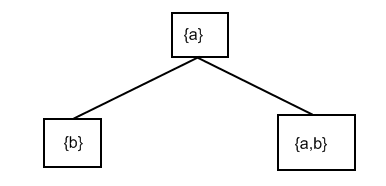
\includegraphics[width=101mm]{tree_1.png}
	\label{fig:tree_1}
\end{figure}

then if we want to add to that tree the root list $\left\{a, c\right\}$ then we end up with the following tree.
\begin{figure}[H]
	\centering
		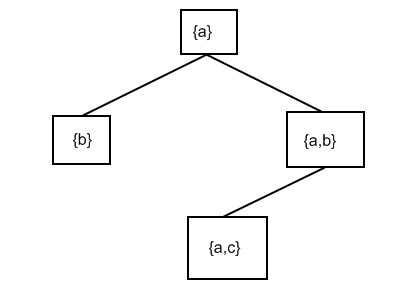
\includegraphics[width=101mm]{tree_2.png}
	\label{fig:tree_2}
\end{figure}

Adding and searching in binary trees takes order $O(log_2(n))$ where n is the number of element in the tree. For large numbers of elements this is substantially better than the equivalent $O(n)$ that one gets from linear linked lists hence justifying the need for the extra data structure over the graph.

We can now discuss the algorithm used to generate the automaton. It takes as input the minimal root list generated previously. From this it does the following:

Begin the automaton with an empty state (a state with empty root list).

\begin{algorithmic}[1]
	\REQUIRE current state as input
	\FOR{each generator $a \in \Sigma$}
		\IF{$a$ is in the root list for the state}
			\STATE This is a fail state so do not store it (there will be a null pointer to here in the code)
		\ELSE
			\STATE create a new state by doing the action of $a$ on each root in the root list of the current state.
			\STATE Add the simple root $v_a$ to the root list just generated.
			\IF{new state exists}
				\STATE Add a link from the current state to the existing one on the path by the generator $a$.
			\ELSE
				\STATE Add the new state to the binary tree of states.
				\STATE Add a link from the current state to the new one.
				\STATE Call this function again with the new state as input parameter.
			\ENDIF
		\ENDIF
	\ENDFOR
\end{algorithmic}

After this function has run its course we have a complete automaton with circuits etc which can be used to detect reduced words and indeed using the work in the previous section can be used to find the reduced form for words. In fact for finite groups it is a simple job to print all the possible words using this automaton.

It is simple, once the automaton is created, to test whether a word is reduced. We simply pass the word to the automaton generator by generator and if we hit a null pointer then we have reached a fail state and the word is not reduced. We can then reduce it using the work in the previous section. Simply testing if a word is reduced can be done in linear time and it is trivial to note that reducing a word is going to be a worst quadratic in the number of characters making up the word. Therefore the majority of the complexity (as expected) comes from creating the automaton.

As promised in the previous section we now continue the example for the group $I_2(\infty)$ (this is the infinite dihedral group).

\begin{example}
	In example \ref{dihedral_inf_example} we found that the minimal root table for the group $W = I_2(\infty)$ is equal to $\left\{v_a, v_b \right\}$. With this in mind we can create the automaton as above.
	
	Begin with the empty state and the generator $a$. The following diagram shows the automaton after each state has been added.
	
	\begin{figure}[H]
		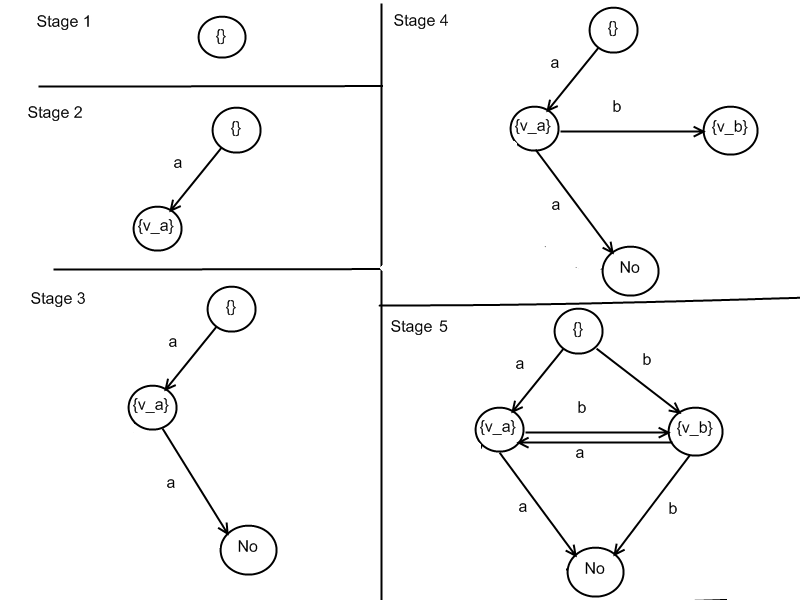
\includegraphics[width=\columnwidth]{inf_dihed_automaton}
	\end{figure}
	
	Stage 5 fills in the remaining connections between the automaton states but in reality this would be split over a few calculations.
	
	Note in particular that in stage 4 the generator $b$ is applied to the set of roots $\left\{v_a\right\}$. This gives us the root $v_a + 2v_b$ which we discard because it isn't minimal. The same happens when we apply $a$ to the root list with $v_b$ in it.
	
	We can also see that not every combination of the roots is in the automaton i.e. the automaton does not have a state in it for the list $\left\{v_a, v_b\right\}$. This is not a mistake, it is simply an effect of the way in which the automaton is generated.
\end{example}

	With that example we conclude this section of the project and note that we have achieved our aim. We are now capable (as was just demonstrated) of creating a finite state automaton for infinite coxeter groups which detects whether a word is reduced. In addition to that we also discussed and proved how these words could be reduced in quadratic time. The final section presents some of the questions which have been left unanswered so far as extension work.

\section{Extension Work}
In the above work we make use of floating point calculations to calculate a variety of things throughout the algorithms. Mathematically there is nothing wrong with these calculations and in practice it is unlikely that any issues will come up. However, computers cannot completely represent non-integer numbers and as we will see this could potentially give some problems.

Let's say that via some chance of the root calculation algorithms we arrive at two roots which differ by less than some number $\epsilon$. In our code at the moment we would treat those roots as being identical and the program would continue computation giving some potential errors later on.

Since the original paper by Brink and Howlett \cite{brinkhowlett93} there has been a small amount of work on the subject which led to the discovery that all of these algorithms can be done without performing any explicit calculation. This would be an excellent extension to this project had there been enough time, in reality we have made do with a constant that controls the amount by which roots are allowed to differ. For a discussion on this topic consider the following paper by Cassleman \cite{casselman08}.

Brink has also published a paper giving a lot more detail about the size and structure of the set of minimal roots. Some of this could be used to sensibly bound the minimal root table and thus the automaton. This can be found in her paper \cite{brinkresearch} or a paper of the same name but with different content published in the journal of algebra \cite{brinkjournal94}. Again this would make interesting reading and potentially provide mechanisms by which the general approach used here could be improved.

\bibliographystyle{plain}
\bibliography{coxeter}

\end{document}